Machine learning is the study of algorithms and 
statistical models employed by computing systems
capable of performing tasks without explicit instruction.
While traditional algorithms rely on some specified input 
and a ruleset for determining the output, machine learning
is instead concerned with a set of generic algorithms which can find patterns
in a broad class of data sets.
This section will give a brief overview of machine learning,
and more specifically the class of algorithms known as neural networks,
and will follow closely the review by
\parencite[Mehta et al.][pages 1-64]{mehta2019high}
which the reader is encouraged to seek out for further information.
\par
Examples of machine learning problems include identifying objects in images,
transcribing text from audio and making film recommendations to viewers 
based on their watch history.
Machine learning problems are often subdivided into 
estimation and prediction problems.
In both cases, we choose some observable 
$\bm{x}$ (e.g. the period of a pendulum)
related to some parameters $\bm{\theta}$ 
(e.g. the length and the gravitational constant)
through a model $p(\bm{x} \lvert \bm{\theta})$ 
that describes the probability of observing
$\bm{x}$ given $\bm{\theta}$. 
Subsequently we perform an experiment to obtain a dataset
$\bm{X}$ and use these data to fit the model. 
Fitting the model means finding the parameters 
$\hat{\bm{\theta}}$ that provide the best explanation for the data. 
\textit{Estimation} problems are concerned with the accuracy of 
$\hat{\bm{\theta}}$, whereas prediction problems are concerned with 
the ability of the model $p(\bm{x} \lvert \bm{\theta})$
to make new predictions.
Physics has traditionally been more concerned with the estimation 
of model parameters, while in this thesis we will be focused 
on the accuracy of the model.
\par
Many problems in machine learning are defined by the same set of ingredients.
The first is the dataset $\mathcal{D} = (\bm{X}, \bm{Y})$,
where $\bm{X}$ is a matrix containing observations of the 
independent variables $\bm{x}$, and $\bm{Y}$ is a matrix containing
observations of dependent variables.
Second is a model $\bm{F}: \bm{x} \rightarrow \bm{y}$
which is a function of the parameters $\bm{\theta}$. 
Finally we have a cost function
$\mathcal{C}\left(\bm{Y}, \bm{F}\left(\bm{X} ; \bm{\theta}\right)\right)$
that judges the performance of our model at generating predictions.
\newline
In the case of linear regression we consider a set of independent observations
$ \bm{X} = 
\begin{bmatrix}
\bm{x}_1 & \bm{x}_2 & \dots & \bm{x}_N
\end{bmatrix}
$
related to a set of dependent observations $\bm{y} = (y_1, y_2, \dots,y_N)$
through a linear model 
$f(\bm{x} ; \bm{\theta}) = 
x_1\cdot w_1 + x_2\cdot w_2 + \dots + x_P\cdot w_P$,
with parameters $\bm{\theta} = (w_1, w_2, \dots,w_P)$. 
The cost function is the well known sum of least squares 
$\mathcal{C}(\bm{y}, f(\bm{X} ; \bm{\theta}))
= \sum_i^N (y_i - f(\bm{x}_i ; \bm{\theta}))^2 $
and the best fit is chosen as the set
of parameters which minimize this cost function: 
$\hat{\bm{\theta}} = \underset{\bm{\theta}}
{\text{argmin}} \ \mathcal{C}(\bm{Y}, f(\bm{X} ; \bm{\theta})) $.

\subsection{Basics of statistical learning}
% needs revision?
Statistical learning theory is a field of statistics dealing with the problem
of making predictions from data. We start with an unknown function \newline
$y = f(x)$ and our goal is to develop a function $h(x)$
such that $h \sim f$. We fix a hypothesis set $\mathcal{H}$ that the
algorithm is willing to consider. The expected error of a particular $h$
over all possible inputs $x$ and outputs $y$ is:

\begin{equation}
 E[h] = \int_{X \times Y} \mathcal{C}(h(x), y) \rho(x,y) dx dy ,
\end{equation}

where $\mathcal{C}$ is a cost function and $\rho(x,y)$ is the joint probability
distribution for $x$ and $y$. This is known as the \textit{expected error}.
Since this is impossible to compute without knowledge of the probability distribution
$\rho$, we instead turn to the \textit{empirical error}. Given $n$ data points
the empirical error is given as:

\begin{equation}
 E_S[h] = \frac{1}{n} \sum_i^n \mathcal{C}(h(x_i), y_i) .
\end{equation}

The \textit{generalization error} is defined as the difference
between the expected and empirical errors:

\begin{equation}
 G = E[h] - E_S[h] .
\end{equation}

We say an algorithm is able to learn from data or \textit{generalize} if 

\begin{equation}
 \lim_{n\to\infty} G = 0 .
\end{equation}

We are in general unable to compute the expected error, and therefore unable
to compute the generalization error. The most common approach known as
\textit{cross-validation} is to estimate the
generalization error by subdividing our dataset into a \textit{training} set
and a \textit{test} set. The value of the cost function on the training set
is called the \textit{in-sample} error and the value of the cost
function on the test set the \textit{out-of-sample} error.
Assuming the dataset is sufficiently large and representative of $f$, and the subsampling
into train and test datasets is unbiased, the in-sample error
can serve as an appropriate proxy for the generalization error.
\newline
In figure \ref{fig:in-out}
we show the typical evolution of the errors as the number of data points increase.
It is assumed that the function being learned is sufficiently complicated
that we cannot learn it exactly, and that we have a sizeable number of data points
available. The in-sample error will decrease monotonically, as our model
is not able to learn the underlying data exactly. In contrast, the out-of-sample
error will decrease, as the sampling noise decreases and the training
data set becomes more representative of the underlying probability distribution.
In the limit, these errors both approach same value, which is known the model
\textit{bias}. The bias represents the best our model could do in the infinite data limit.
The out-of-sample error produced from the sampling noise
is known as \textit{variance}, and will vanish completely
given an infinite representative data set.

% create own figures or cite properly
\begin{figure}[h]
    \centering
    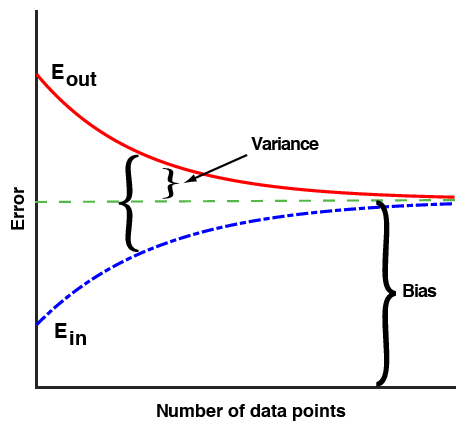
\includegraphics[width=0.75\linewidth]{in-out-sample.png}
    \caption{Typical in-sample and out-of-sample error as a function
    of the number of data points. It is assumed that the number
    of data points is not small, and that the true function
    cannot be exactly fit.}
    \label{fig:in-out}
\end{figure}

In figure \ref{fig:bias-variance} we show the typical evolution
of the out-of-sample error as the model \textit{complexity} increases.
Model complexity is a measure of the degrees of freedom in the model space,
for example the number of coefficients in a polynomial regression.
In the figure we can see that bias decreases monotonically as model complexity
increases, as the model is able to fit a larger space of functions.
However, the variance will also increase as the model becomes more
susceptible to sampling noise. In general the lowest out-of-sample error,
and therefore generalization error, is achieved at an intermediate
model complexity. We also find that as model complexity increases,
a larger amount of data points is required to be able to reasonably
fit the true function.

% create own figures or cite properly
\begin{figure}[h]
    \centering
    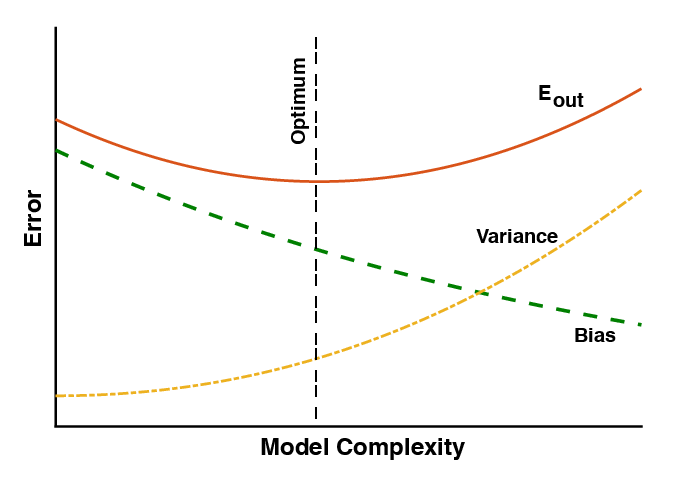
\includegraphics[width=0.75\linewidth]{bias-variance.png}
    \caption{Typical out-of-sample error as a function
    of model complexity for a fixed dataset. Bias decreases monotonically with
    model complexity, while variance increases as a result of
    sampling noise.}
    \label{fig:bias-variance}
\end{figure}

\subsection{Bias-variance decomposition}
Consider a dataset $\mathcal{D}(\bm{X}, \bm{y})$ of $n$ pairs
of independent and dependent variables. Assume the true data
is generated from a noisy model:

\begin{equation}
 y = f(\bm{x}) + \epsilon ,
\end{equation}

where $\epsilon$ is normally distributed with mean $\mu$ and
standard deviation $\sigma$. Assume that we have an estimator $h(\bm{x}; \bm{\theta})$
trained by minimizing a cost function $\mathcal{C}(\bm{y}, h(\bm{x}))$
which we take to be the sum of squared errors:

\begin{equation}
 \mathcal{C}(\bm{y}, h(\bm{x})) = \sum_i^n (y_i - h(\bm{x}_i; \bm{\theta}))^2 .
\end{equation}

Our best estimate for the model parameters:

\begin{equation}
 \bm{\theta}_{\mathcal{D}} = \underset{\bm{\theta}}{\argmin} \
\mathcal{C}(\bm{y}, h(\bm{x}; \bm{\theta})) ,
\end{equation}

is a function of the dataset $\mathcal{D}$. If we imagine we have a set of
datasets $\mathcal{D}_j = (\bm{y}_j, \bm{X}_j)$, each with $n$ samples, we would like to calculate
the expectation value of the cost function over all these datasets $E_{\mathcal{D}, \epsilon}$.
We would also like to calculate the expectation value over different instances of the noise $\epsilon$.
The expected generalization error can be decomposed as:
% more in depth?
\begin{equation}
\begin{split}
    E_{\mathcal{D}, \epsilon} [\mathcal{C}(\bm{y}, h(\bm{X} ; \bm{\theta}_{\mathcal{D}}))]
    &= E \left[ \sum_i (y_i - h(\bm{x}_i ; \bm{\theta}_{\mathcal{D}}))^2 \right] \\
    &= \sum_i \sigma_{\epsilon}^2 + E_{\mathcal{D}}[(f(\bm{x}_i) - f(\bm{x}_i ; \bm{\theta}_{\mathcal{D}}))^2] .
\end{split}
\end{equation}

The second term can be further decomposed as
\begin{equation}
\begin{split}
    &E_{\mathcal{D}}[(f(\bm{x}_i) - f(\bm{x}_i ; \bm{\theta}_{\mathcal{D}}))^2] \\
    &= (f(\bm{x}_i) - E_{\mathcal{D}}[h(\bm{x}_i ; \bm{\theta}_{\mathcal{D}})])^2
    + E[(h(\bm{x}_i ; \bm{\theta}_{\mathcal{D}}) - E[h(\bm{x}_i ; \bm{\theta}_{\mathcal{D}}])^2]
\end{split}
\end{equation}

The first term is what we have referred to as the bias:

\begin{equation}
    \text{Bias}^2 = \sum_i (f(\bm{x}_i) - E_{\mathcal{D}}[h(\bm{x}_i ; \bm{\theta}_{\mathcal{D}})])^2.
\end{equation}

The bias measures the expectation value of the deviation of our model from the true
function, i.e. the best we can do in the infinite data limit.
\newline
The second term is what we have referred to as the variance:
\begin{equation}
    \text{Var} = \sum_i  E[(h(\bm{x}_i ; \bm{\theta}_{\mathcal{D}}) - E[h(\bm{x}_i ; \bm{\theta}_{\mathcal{D}}])^2]
\end{equation}

The variance measures the deviation of our model due to finite-sampling effects.
Combining these effects we can decompose the out-of-sample error into:
\begin{equation}
    E_{\text{out}} = \text{Bias}^2 + \text{Var} + \text{Noise},
\end{equation}

with $\text{Noise} = \sum_i \sigma_{\epsilon}^2$.
\newline
In general it can be much more difficult to obtain sufficient good data
than to train a very complex model. Therefore it is often useful in practice
to use a less complex model with higher bias, because it is less susceptible
to finite-sampling effects.

\subsection{Neural networks}
Artificial Neural Networks (ANN) or Deep Neural Networks (DNN) are
supervised learning models vaguely inspired by biological neural networks.
The building blocks of neural networks are neurons that take a
vector input of $d$ features $\bm{x} = (x_1,\dots,x_d)$
and produce a scalar output $a(\bm{x})$.
A neural networks consists of layers of these neurons stacked together
with the output of one layer serving as input for another. The
first layer is typically known as the \textit{input layer}, the
middle layers as \textit{hidden layers} and the final layer
the \textit{output layer}. The basic architecture is shown in
figure \ref{fig:neural-networks}.
In almost all cases the output $a_i(\bm{x})$ of neuron $i$ can be decomposed
into a linear operation on the inputs passed through a non-linear
activation function:

\begin{equation}
 a_i(\bm{x}) = \sigma_i(z_i) ,
\end{equation}

where $\sigma_i$ is a non-linear function and $z_i$
is the dot product between the inputs $\bm{x}$ and a set of
neuron-specific weights $\bm{w}_i$:

\begin{equation}
 z_i = \bm{x}^T \bm{w}_i + b_i .
\end{equation}

The term $b_i$ is a neuron-specific re-centering of the input.
\newline
Typical choices of non-linearities/activation functions include
the sigmoid and hyperbolic tangent functions, and Rectified Linear Units (ReLU).
When the activation function is non-linear, the neural network with a single hidden
layer can be proven to be a \textit{universal function approximator},
given an arbitrarily large number of neurons. We typically also
want functions that are monotonic and smooth with a monotonic derivative.
\newline

% own figure or cite
\begin{figure}[h]
    \centering
    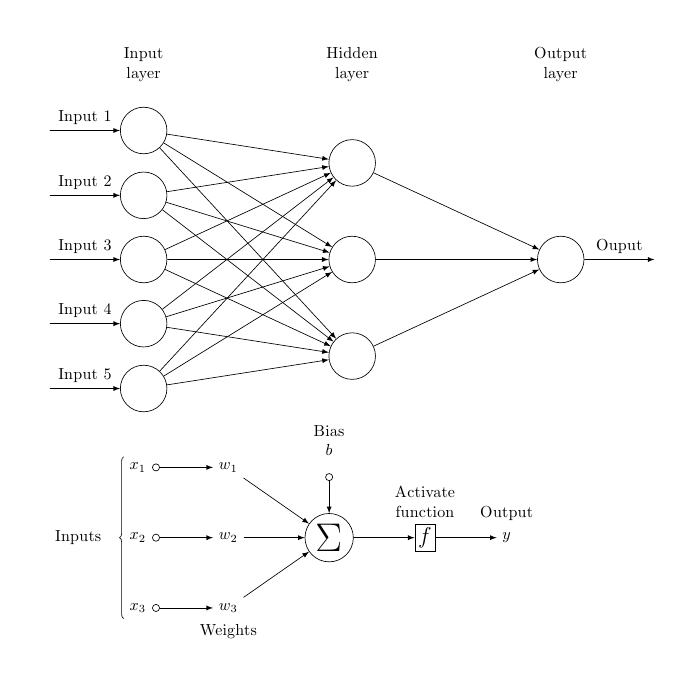
\includegraphics[width=0.75\linewidth]{neural-networks.png}
    \caption{Text.}
    \label{fig:neural-networks}
\end{figure}

The simplest neural networks are known as \textit{feed-forward} neural networks (FNN).
The input layer is the vector $\bm{x}$ of inputs, while each neuron in the first
hidden layer performs a dot product between its weights $\bm{w}_i$ and the inputs
and passes it through a non-linearity $\sigma_i$. The activation function
is typically shared across one or multiple layers $\sigma_i = \sigma$. The vector of neuron outputs
$\bm{a}_i$ serves as input to the next hidden layer until we reach the final layer.
In the final layer the choice of activation function is dependent on the problem
we are trying to solve. If we are performing non-linear regression the
final activation function is often the identity $\sigma_i(z) = z$, or if
we are doing classification the soft-max function is often employed.

\newpage

Let $\bm{x}$ be a vector of $d = 1,\dots,D$ inputs or 
\textit{features}. Let $a_i^{(h)}$
denote the output of neuron $i = 1,\dots,N_l$ in layer $l = 1,\dots,L$.
The output of neuron $i$ in the first hidden layer $a_i^{(1)}$ is thus:

\begin{equation}
\begin{split}
    z_i^{(1)} &= \bm{x}^T \bm{w}_i^{(1)} + b_i^{(1)} , \\
    a_i^{(1)} &= \sigma_i^{(1)}(z_i^{(1)}) . 
\end{split}
\end{equation}

The inputs are iterated through each hidden layer until we reach the final layer.
Denote the vector of outputs $\bm{o} = \left(o_1,\dots,o_O\right)$:

\begin{equation}
\begin{split}
    z_i^{(L)} &= (\bm{a}_{L-1})^T \bm{w}_i^{(L)} + b_i^{(L)} , \\
    a_i^{(L)} &= o_i \\
              &= \sigma_i^{(L)}(z_i^{(L)}) \\
    &= \sigma_i^{(L)} \left((\bm{a}_{L-1})^T \bm{w}_i^{(L)} + b_i^{(L)} \right) \\
    &= \sigma_i^{(L)} \left(
    \left( \sigma_1^{(L-1)},\dots,\sigma_{N_{L-1}}^{(L-1)} \right)^T
    \bm{w}_i^{(L)} + b_i^{(L)} \right) .
\end{split}
\end{equation}

This allows us to compose a complicated function $\bm{F}: \mathbb{R}^D \rightarrow
\mathbb{R}^O$, with $D$ the number of inputs and $O$ the number of outputs.
The \textit{universal approximation theorem} tells us that this simple architecture
can approximate any of a large set of continuous functions
given appropriate choice of weights $\bm{w}_i^h$ and mild assumptions
on the activation functions. The theorem requires only a single hidden layer,
where the strength of the approximation relies on the number of neurons.
In practice it has been found that adding more layers produces
faster convergence and higher accuracy, which has given rise
to the field of \textit{deep learning}.

\subsection{Backpropagation}
Given a set of datapoints $(\bm{x}_i, y_i), \ i=1,\dots,n$,
the value of the cost function is entirely determined
by the weights and biases of each neuron in the network.
We define learning narrowly as adjusting the parameters of the network
in order to minimize the cost function.
\newline
\textit{Gradient descent} is a simple, but powerful method
of finding the minima of differentiable functions.
Given a function $F: \mathbb{R}^d \rightarrow \mathbb{R}$, and an initial
value $\bm{x}_0$ we define an iterative procedure:

\begin{equation}
 \bm{x}_{n+1} = \bm{x}_{n} - \eta \nabla F(\bm{x}_n), 
\end{equation}

where $\eta$ is known as the \textit{learning rate}.
The procedure terminates when the norm
$ \left| \nabla F(\bm{x}_n) \right| $ or
$ \left| x_{n+1} - x_{n} \right| $
is appropriately small.
\newline
The learning rate is not necessarily fixed throughout the procedure,
and proves crucial to the convergence of the method. If $f$
is convex, and $\eta$ is reasonably small, convergence is guaranteed.
Convergence may be very slow however, and if $f$ is not convex
you are only guaranteed to find local minima, and this makes
the method very sensitive to initial conditions.
\par
In order to train the model, we need to calculate the derivative of the cost
function with respect to a very large number of parameters multiple times. However,
numerical calculation of gradients is very time consuming. The \textit{backpropagation}
algorithm is a clever use of the chain rule that allows us to calculate gradients efficiently.
\par
Assume that there are $L$ layers in our network with $l = 1,2,...,L$ indexing the layers, including
the output layer and all the hidden layers.
Let $w_{ij}^l$ denote the weight for the connection
from the $i$-th neuron in layer $l - 1$ to the $j$-th neuron in layer $l$. Let $b_{j}^l$ denote the bias of this $j$-th neuron.

The activation $a_{j}^l$ of the $j$-th neuron in the $l$-th layer is related to the activities of the neurons in the layer $l - 1$ by:

\begin{equation}
 a_{j}^l = f \left( \sum_i w_{ij}^l a_i^{l-1} + b_j^l \right) = f \left( z_j^l \right) ,
\end{equation}

where $f$ is some activation function.

The cost function $\mathcal{C}$ depends directly on the activations in the output layer, and indirectly on the activations
in all the lower layers.
Define the error $\Delta_j^L$ of the $j$-th neuron in the $L$-th (final) layer as the change in cost function
with respect to the weighted input $z_j^L$:

\begin{equation}
 \Delta_j^L = \frac{\partial \mathcal{C}}{\partial z_j^L} .
\end{equation}

Define analogously the error $\Delta_j^l$ of neuron $j$ in the $l$-th layer as the change in cost function with respect to the weighted input
$z_j^l$:

\begin{equation}
 \Delta_j^l = \frac{\partial \mathcal{C}}{\partial z_j^l} .
\end{equation}

This can also be interpreted as the change in cost function with respect to the bias $b_j^l$:

\begin{equation}
 \Delta_j^l = \frac{\partial \mathcal{C}}{\partial z_j^l} = \frac{\partial \mathcal{C}}{\partial b_j^l} 
\frac{\partial b_j^l}{\partial z_j^l} = \frac{\partial \mathcal{C}}{\partial b_j^l} ,
\end{equation}

since $ \partial b_l^j / \partial z_j^l = 1$.

The error depends on neurons in layer $l$ only through the 
activation of neurons in layer $l + 1$, so using the chain rule we can write:

\begin{equation}\label{eq:error}
\begin{split}
\Delta_j^l &= \frac{\partial \mathcal{C}}{\partial z_j^l} = \sum_i \frac{\partial \mathcal{C}}{\partial z_i^{l+1}}
\frac{\partial z_i^{l+1}}{\partial z_j^l} \\
           &= \sum_i \Delta_i^{l+1} \frac{\partial z_i^{l+1}}{\partial z_j^l} \\
           &= \sum_i \Delta_i^{l+1} w_{ij}^{l+1} f'(z_j^l) \\
           &= \left( \sum_i \Delta_i^{l+1} w_{ij}^{l+1} \right) f'(z_j^l) .\\
\end{split}
\end{equation}

The sum comes from the fact that any error in neuron $j$ in the $l$-th layer propagates to all the neurons
in the layer $l + 1$,
so we have to sum up these errors.

This gives us the equations we need to update the weights and biases of our network:

\begin{equation}
 \frac{\partial \mathcal{C}}{\partial w_{ij}^l} 
= \frac{\partial \mathcal{C}}{\partial z_j^l} 
\frac{\partial z_j^l}{\partial w_{ij}^l}
= \Delta_j^l a_i^{l-1} .
\end{equation}

\begin{equation}
 \frac{\partial \mathcal{C}}{\partial b_{j}^l} = \Delta_j^l .
\end{equation}

Now, if we have the error of every neuron $j$ at the output layer,
$\Delta_j^L$, equation \ref{eq:error}
gives us the recipe for calculating the error in the preceding layer until we reach the first hidden layer, 
and we are done. All we are missing is the error at the output layer:

\begin{equation}
\Delta_j^L = \frac{\partial \mathcal{C}}{\partial z_j^L} 
= \frac{\partial}{\partial z_j^L} \left(
    \sum_o \frac{1}{2}\left( z_o^L - y_o\right)^2 \right) 
    = z_j^L - y_j .
\end{equation}

Now, since the derivatives for the weights depend on
the activations in the preceding layer, this suggests
an iterative procedure for training the network.
First we feed the input data through the network
and obtain activations and an output, then these
outputs are backpropagated through the network to update the
weights and biases. This is then repeated for some number
of steps or until the network achieves acceptable accuracy.

% own figure or cite properly
\begin{figure}
    \centering
    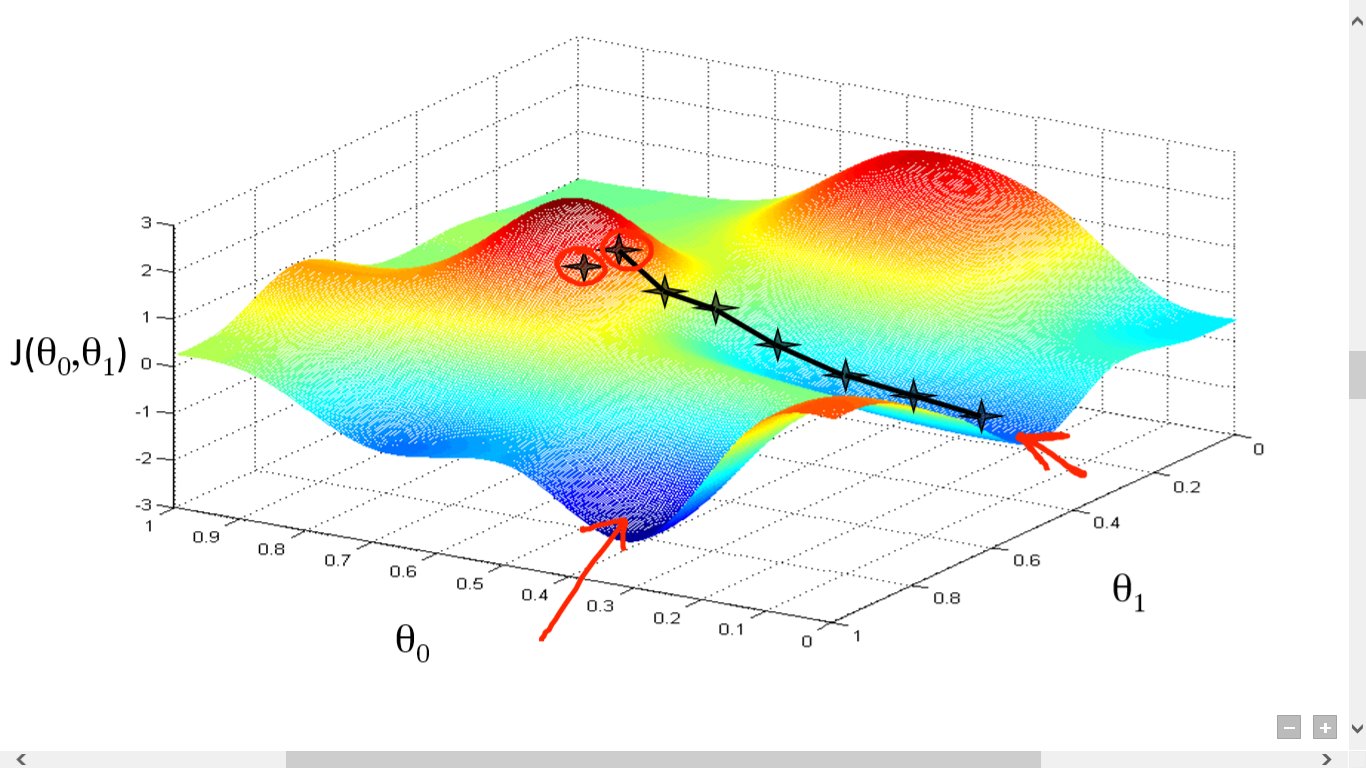
\includegraphics[width=0.75\linewidth]{gradient-descent.png}
    \caption{Text.}
    \label{fig:gradient-descent}
\end{figure}

\subsection{Optimization}
In order to begin the minimization procedure and find an optimal
set of weights and biases for our network we first need some initial values.
Often weights are initialized with small values distributed around zero,
drawn from a uniform or normal distribution. The bias can be initalized to zero,
but enforcing that all biases have some small value ensures that every
neuron has output which can be backpropagated in the first training cycle.
In the Pytorch neural network framework - which is the one we will 
be using - weights are initialized uniformly as

\begin{equation}
    \begin{split}
        \sigma &= 1 / N_{in} \\
        w &= \mathcal{U}(-\sigma, \sigma)
    \end{split}
\end{equation}

where $N_{in}$ is the number of inputs to the weight/layer of weights
and $\mathcal{U}$ is the uniform distribution.
\par
A critical choice for building neural networks is the choice of activation function.
As we have mentioned briefly above, we have a small set of requirements in order
for the neural network to be an universal function approximator, namely
that the function be nonconstant, bounded, continuous and monotonically increasing.
We also desire that the function be fast to evaluate, with a derivative that
is simple to calculate.
\par
A function that fulfills all of these criteria is the sigmoid function:

\begin{equation}
    \begin{split}
        \sigma(x) &= \frac{1}{1 + e^{-x}} , \\
        \sigma '(x) &= \sigma(x)(1 - \sigma(x)) .
    \end{split}
\end{equation}

The sigmoid function is defined on the entire real number line,
and outputs a number between $0$ and $1$. It also has a continuous derivative
which is simple to calculate. The sigmoid function is well suited for binary
classifiers, since it easily creates a decision boundary between two categories
$0$ and $1$, and is often the first goto for AI programmers.
\par
Another simple and commonly used activation function is the hyperbolic tangent

\begin{equation}
    \begin{split}
        \tanh(x) &= \frac{e^{2x} -1}{e^{2x} - 1} , \\
        \tanh '(x) &= (1 - \tanh(x)^2) .
    \end{split}
\end{equation}

The hyperbolic tangent is defined on the real number line and outputs
a number between $-1$ and $1$.
\par
Both the sigmoid and the hyperbolic tangent functions exhibit the problem
of vanishing gradients. In deep learning, you typically have several layers
of neurons outputting some linear combination of the activation functions.
Through the backpropagation algorithm, each neuron receives a weight update
proportional to the partial derivative of the loss with respect to
its weights. For the sigmoid and hyperbolic tangent activations these
gradients will be in the range $(-1, 1)$, and therefore often
exceedingly small. This means that many neurons may receive effectively
no weight update in any given training epoch, which severely impedes training.
\par
The Rectified Linear Unit (ReLU) has gained popularity in recent years
for its effectiveness in the field of convolutional neural networks.
The ReLu function is defined as:

\begin{equation}
    \begin{split}
        \text{ReLU}(x) &=
    \begin{cases}
        x & x \geq 0 \\
        0 & x < 0
    \end{cases} \\
        \text{ReLU}'(x) &=
    \begin{cases}
        1 & x \geq 0 \\
        0 & x < 0
    \end{cases}
    \end{split}
\end{equation}

Since the ReLU function in principle has no upper bound, it does
not suffer the effect of vanishing gradients. Instead, the ReLU function
can produce exploding gradients, if one or more activations becomes
very large. In practice the gradients are often "clipped", i.e.
truncated above a certain upper bound.
With the ReLU function one can also encounter "dying" neurons,
since the input to any neuron that does not exceed zero
is set to zero, which means that the number of neurons receiving
an effective weight update
\newline
\newline
From the point of view of the neural network, the inputs are just
dimensionless numbers, which are passed through layers until it spits
out some outputs. It is therefore often useful to standardize the inputs.
A common method is to shift the inputs by their mean and
normalize by their standard deviation:

\begin{equation}
 x_{i}' = \frac{x_{i} - \bar{x}}{\sigma_x} . 
\end{equation}

This is often useful in speeding up the training of neural networks.
In theory any shifting and rescaling can be reproduced simply
by updating the weights and biases of the network.
In practice however, as the weights often start as
small numbers, it can take quite a few training cycles before
the weights are of appropriate size.
Standardizing the inputs also makes it impose to
impose a penalty on the weights in order to reduce
overfitting.
\newline
\newline
The most common methods for training neural networks
are variations on the simple gradient descent scheme as mentioned
above:

\begin{equation}
 \bm{x}_{n+1} = \bm{x}_{n} - \eta \nabla F(\bm{x}_n) . 
\end{equation}

Since we are interested in training neural networks,
$\bm{x}_{n}$ represents the weights and biases of the network
after $n$ training cycles, $\eta$ is our learning rate
and $\nabla F(\bm{x}_n)$ is the gradient of the loss function.
\par
The learning rate $\eta$ controls how fast we reach a given minimum.
A small learning rate will require more training cycles
and a larger learning rate will require fewer.
The learning rate also controls the numerical stability
of the method, if it is too large the weights may diverge
and if it is too small the weight may never converge.
Gradient descent also tends to exhibit oscillating behaviour
around the minimum. Often a schedule is imposed
on the learning rate, such as reducing it by a fixed amount
every few epochs or incorporating an exponentially decaying learning rate.
[cite: Mehta et al]
As discussed in Mehta et. al. using gradient descent to optimize
our neural network imposes some limitations:

\begin{itemize}
    \item \textit{Gradient descent finds local minima} - 
        if the GD algorithm converges, it will converge to
        a local minimum. This can lead to poor performance
        in complicated cost function landscapes
    \item \textit{Gradients are expensive to compute} - 
        the loss function often includes a term for each
        data point, which means the gradient also does.
    \item \textit{GD is sensitive to learning rate} - 
        as mentioned above, GD is very sensitive to
        learning rate
    \item \textit{GD is sensitive to initial conditions} - 
        gradient descent can take two different initial values
        and converge at two drastically different values
    \item \textit{GD does not take curvature into account} - 
        the learning rate for gradient descent is the same
        in all directions of parameter space, which means
        the maximum learning rate is set by the behaviour of the
        steepest direction
\end{itemize}

A common method for ameliorating some of these concerns
is minibatching the inputs. Instead of calculating
the gradient on the entire dataset for every epoch,
we instead calculate the gradient on a subset
of the data called a minibatch.
If there are $n$ datapoints and a minibatch size
of $m$ the total number of batches is $n/m$.
If we denote each minibatch $b_k, \ k=1,2,\dots,n/m$
the gradient becomes:

\begin{equation}
 \nabla \mathcal{C} = \frac{1}{n} \sum_{i=1}^N
    \nabla \mathcal{L}_i \rightarrow
    \frac{1}{m} \sum_{i \in b_k} \nabla \mathcal{L}_i , 
\end{equation}

i.e. instead of averaging the loss over the entire dataset
we instead average over a minibatch.
This significantly speeds up the calculation, since
we do not use the entire dataset for every update.
In addition, introducing stochasticity in the
division of the dataset into minibatches introduces stochasticity
to the weights update, which should help gradient descent
in overcoming local minima.
\par
It is also common to introduce regularization to the weights
and biases of the networks. Regularization in the context
of neural networks means adding a term proportional
to the $L_p$ norm of the weights and biases.
For example using the L2-norm our cost function becomes:

\begin{equation}
 \nabla \mathcal{C} = \frac{1}{n} \sum_i \nabla \mathcal{L}_i
    \rightarrow \frac{1}{n} \sum_i \nabla \mathcal{L}_i
    + \lambda \left| \left| \bm{w} \right| \right|^2
    = \frac{1}{n} \sum_i \nabla \mathcal{L}_i
    + \lambda \sum_{ij} w_{ij}^2 , 
\end{equation}

i.e. we sum up all the weights squared.
The parameter $\lambda$ is known as a regularization parameter.
This extra term adds a penalty on the size of the weights
dependant on the regularization parameter. This has
been shown to reduce overfitting, as the weights
cannot be adjusted to arbitrary size in order
to fit the training dataset.
\par
Gradient descent is often paired with a momentum parameter
that serves as a "memory" of the direction we are moving.
This can be implemented as a modification to the
gradient descent update:

\begin{equation}
    \begin{split}
        \bm{v}_n &= \gamma \bm{v}_{n-1} + \eta \nabla F(\bm{x}_n) , \\
        \bm{x}_{n+1} &= \bm{x}_n - \bm{v}_n ,
    \end{split}
\end{equation}

where $0 < \gamma < 1$ is a memory parameter
that controls the time scale for the memory.
It is termed a momentum parameter because the equations
for updating the parameters $\bm{x}$ are analogous to
the equations of motion for a particle moving
in a viscous medium. Momentum helps the gradient descent
algorithm gain speed in directions where the curvature
is flat while dampening speed in high curvature directions.
\par
First-order gradient descent methods differ from quasi-Newton methods
in that they do not keep track of the curvature which is encoded
in the so-called Hessian matrix of second order derivatives.
Second-order methods accomplish this by calculating or approximating
the Hessian and normalizing the learning rate by the curvature.
\par
The RMSprop algorithm keeps a running average of both the
first and second moment of the gradient. If we term
the gradient as $\bm{g} = \nabla F(\bm{x})$
and the first and second orders as
$\bm{m} = \mathbb{E}[\bm{g}]$ and $\bm{s} = \mathbb{E}[\bm{g}^2]$
we can write the update rule as:

\begin{equation}
    \begin{split}
        \bm{g}_n &= \nabla F(\bm{x}_n) \\
        \bm{s}_n &= \beta \bm{s}_{n-1} + (1 - \beta)\bm{g}_{n}^2 \\
        \bm{x}_{n+1} &= \bm{x}_n - \eta \frac{\bm{g}_n}
        {\sqrt{\bm{s}_n + \epsilon}}
    \end{split}
\end{equation}

where $\beta$ is a parameter which controls the time scale
of the averaging and $\epsilon$ is a small regularization constant
to prevent divergences. Operations involving vectors are understood
to be element-wise. This results in a dampening of the learning rate
in directions where the gradient is consistently large,
and allows us to use a larger learning rate for areas
of flat curvature.
\par
Perhaps the most commonly used optimizer today is the closely
related ADAM optimizer. In addition to keeping a running average
of the first and second-order moments ADAM performs
an additional bias correction to account for the 
fact that we are estimating first and second order moments
using a running average. The update rule is given as:

\begin{equation}
    \begin{split}
        \bm{g}_n &= \nabla F(\bm{x}_n) \\
        \bm{m}_n &= \beta_1 \bm{m}_{n-1} + (1 - \beta_1)\bm{g}_n \\
        \bm{s}_n &= \beta_2 \bm{s}_{n-1} + (1 - \beta_2)\bm{g}_n^2 \\
        \hat{\bm{m}}_n &= \frac{\bm{m}_n}{1 - \beta_1^n} \\
        \hat{\bm{s}}_n &= \frac{\bm{s}_n}{1 - \beta_2^n} \\
        \bm{x}_{n+1} &= \bm{x}_n - \eta \frac{\hat{\bm{m}}_n}
        {\sqrt{\hat{\bm{s}}_n} + \epsilon} ,
    \end{split}
\end{equation}

with $\beta_1$ and $\beta_2$ as memory parameters for the first and
second moments respectively. This update rule
effectively normalizes the learning rate by the
standard deviation of the gradient, which is a natural
measurement scale. This also has the effect
of cutting off directions where the gradient varies
by a lot.
